\documentclass{../source/zjureport}

\major{信息工程}
\name{周灿松}
\title{华为云鲲鹏集群搭建}
\stuid{3190105055}
\college{信息与电子工程学院}
\date{\today}
\lab{教7-104}
\course{数据分析与算法设计}
\instructor{赵明敏}
\grades{}
\expname{华为云鲲鹏集群搭建}
\exptype{设计实验}
\partner{}

\begin{document}
    \makecover
    \makeheader
    \section{实验概览}

        \subsection{实验介绍}
        本实验基于华为云OBS和华为云ECS服务构建一个存算分离的基本架构,并通过运行一个计算程序来完成存算分离架构的验证。本实验的实验数据存储在OBS中,通过在ECS上部署开源组件(Hadoop和Spark)构成计算环境,最后编写Spark程序访问存储在OBS上的数据进行计算(单词出现次数统计)并输出结果。

        本实验的基本步骤包含:
        \begin{enumerate}
            \item 购买并配置ECS;
            \item 购买OBS并获取访问密钥AK/SK信息;
            \item 搭建Hadoop集群;
            \item 搭建Spark集群;
            \item 编写Spark程序验证存算分离。
        \end{enumerate}
        \begin{figure}[H]
            \centering
            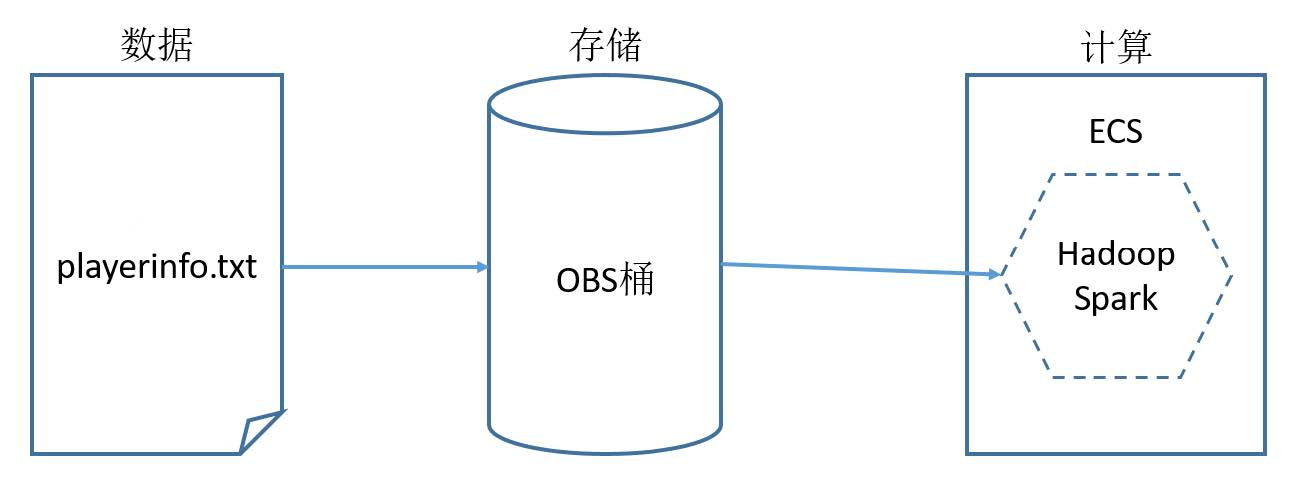
\includegraphics[]{figure/框图.jpg}
        \end{figure}

        \subsection{实验目的}
            \begin{enumerate}
                \item 掌握华为云OBS的购买和使用。
                \item 掌握华为云ECS的购买和使用。
                \item 掌握Hadoop\\Spark环境搭建。
                \item 掌握Spark程序读取OBS数据。
            \end{enumerate}

        \subsection{实验流程}
        \begin{figure}[H]
            \centering
            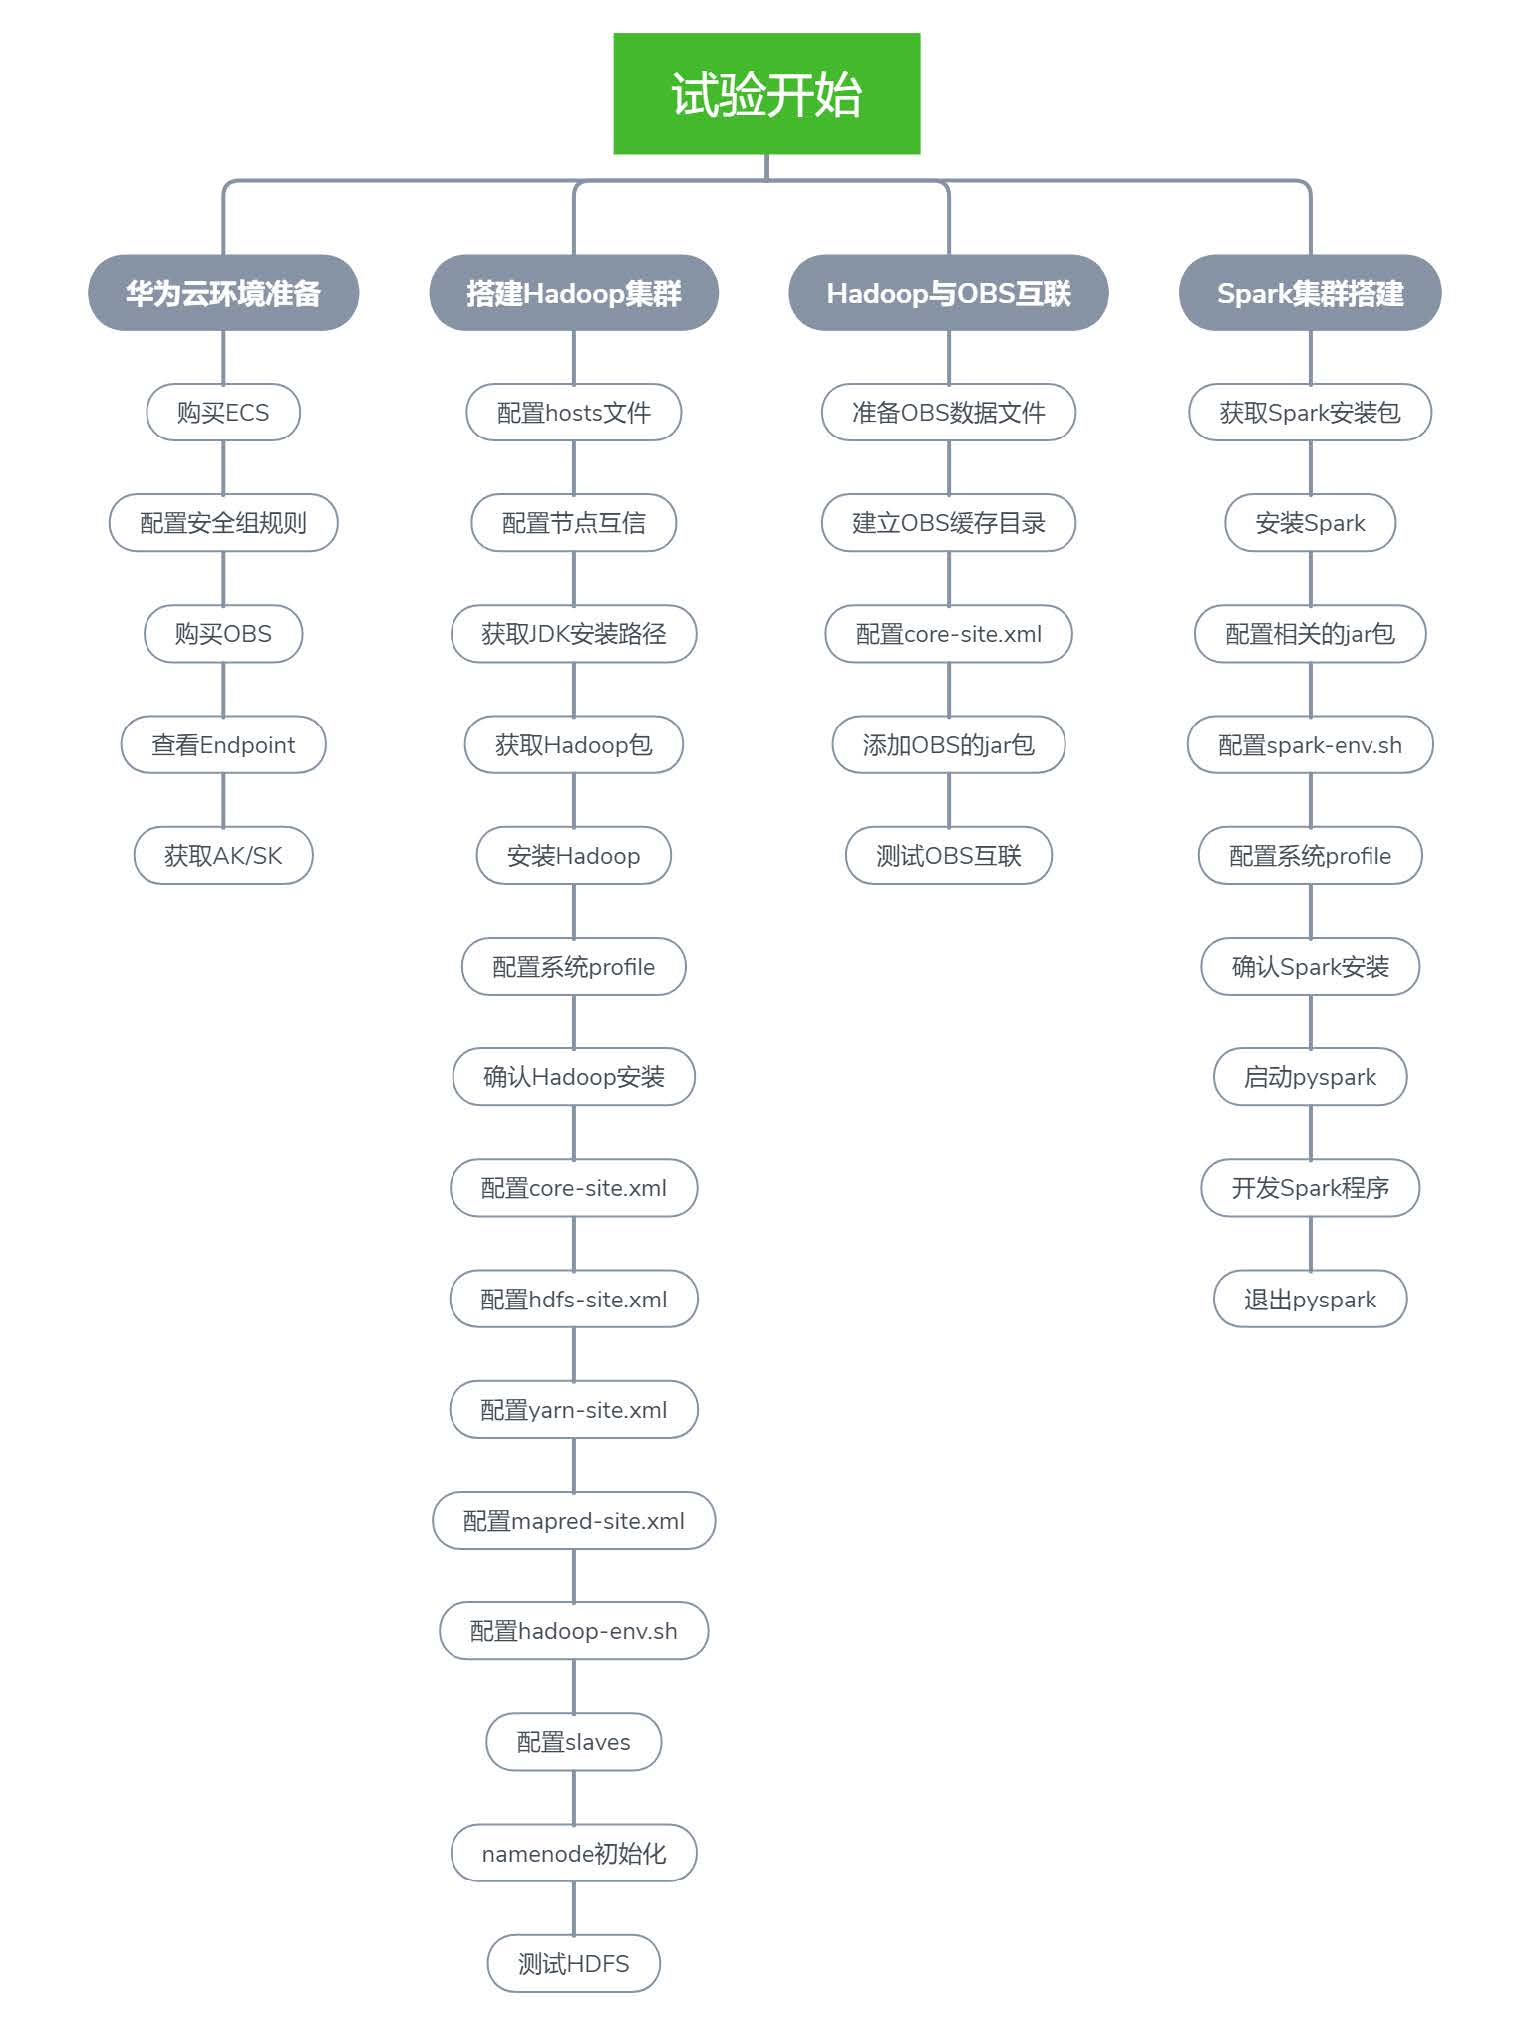
\includegraphics[scale = 0.9]{figure/实验流程.jpg}
        \end{figure}

    \section{华为云环境准备}
        按照实验手册中的方法购买华为云ECS服务器,这里需要注意的一点是需要配置好安全组中的入方向规则。为了方便,和实验手册中一样将所有协议放通并且将规则的优先级设为1使其成为优先级最高的规则。在完成了这一步之后便可以使用远程工具通过ssh连接到云服务器了。
        \begin{figure}[H]
            \centering
            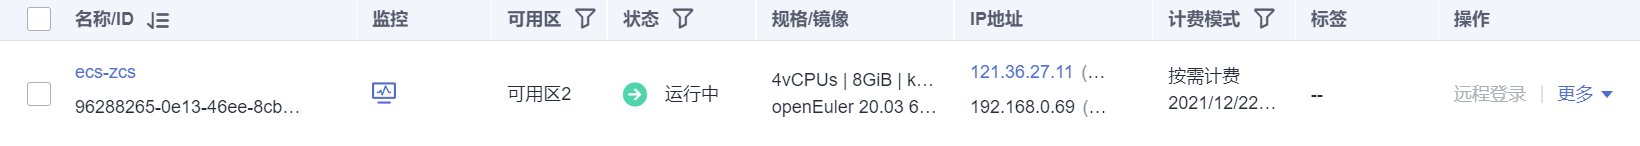
\includegraphics[width = \textwidth]{figure/购买ECS}
            \caption*{购买完成截图}
        \end{figure}

    \section{准备OBS服务}
        \subsection{购买OBS}
        按照实验教程中的步骤进行操作,购买完成截图如下,并记录下endpoint值
        \begin{figure}[H]
            \centering
            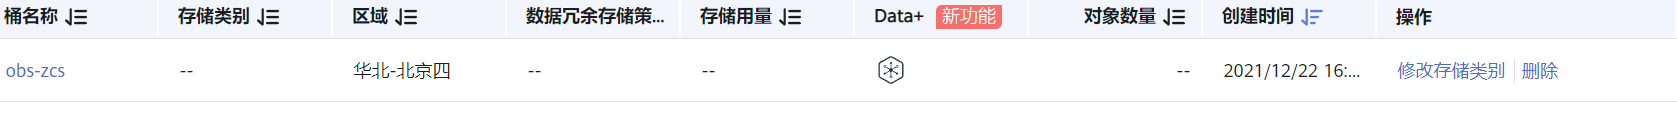
\includegraphics[width = \textwidth]{figure/创建桶.png}
            \caption*{桶创建完成截图}
        \end{figure}

        \subsection{获取访问密钥AK/SK}
        按照实验教程所示操作得到访问密钥,为后续操作做准备

    \section{搭建Hadoop集群}
        \subsection{实验介绍}
            \subsubsection{关于本实验}
            本部分实验需要在已经购买的ECS上搭建Hadoop集群,并且通过配置与华为云OBS服务互联,使Hadoop集群可读取OBS数据。

            \subsubsection{实验目的}
            \begin{enumerate}
                \item 掌握在ECS上搭建Hadoop集群方法
                \item 掌握Hadoop集群与华为云OBS互联方法
            \end{enumerate}

        \subsection{Hadoop集群搭建}
            \subsubsection{配置ECS}
                此处我选择了使用自己比较熟悉的Windows Terminal进行远程连接,方法为在Windows Terminal中输入\bf{ssh root@121.36.27.11},并且输入设置好的密码即可使用root用户登录云端服务器。如图\ref{远程连接}所示
                \begin{figure}[H]
                    \centering
                    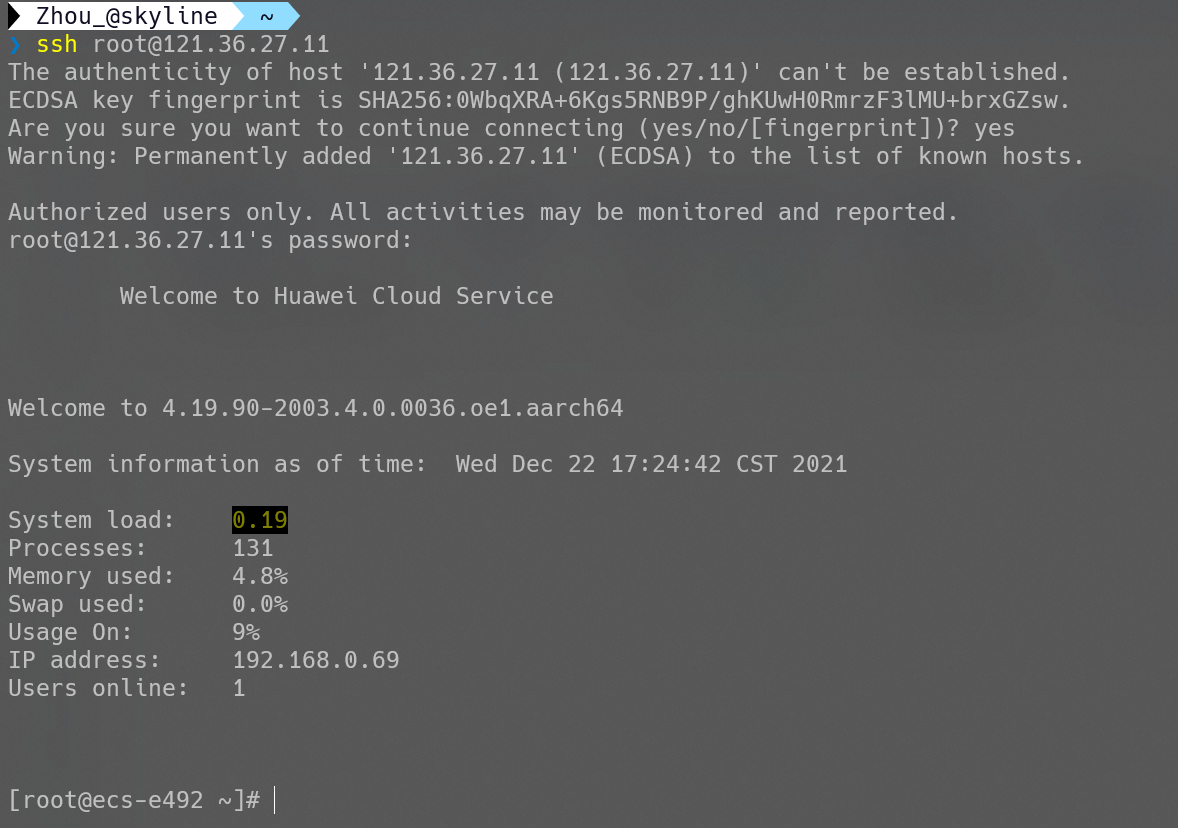
\includegraphics[width = \textwidth]{figure/远程登陆.png}
                    \caption{远程登陆}
                    \label{远程连接}
                \end{figure}

                随后如教程中所示在terminal中通过ssh公钥建立互信节点

            \subsubsection{获取JDK的安装路径}
                按照实验手册中的操作步骤得到JAVA_HOME的值为$\text{/usr/lib/jvm/java-1.8.0-openjdk-1.8.0.242.b08-1.h5.oe1.aarch64}$

        \subsection{搭建Hadoop伪分布式集群}
            \subsubsection{Hadoop安装}
                在安装Hadoop时,实验教程中是直接让云服务器使用wegt工具下载Hadoop的压缩包,但是在这一步时,我发现华为云的网速慢得离谱,仅有12kB/s.下载一个244MB的文件竟然需要15h,这是难以容忍的。在询问相关工作人员无果、网上查阅资料也无法解决的情况下,我选择了在wsl中下载好安装包然后上传到云服务器上的方式解决,如图\ref{上传hadoop}所示。
                \begin{figure}[H]
                    \centering
                    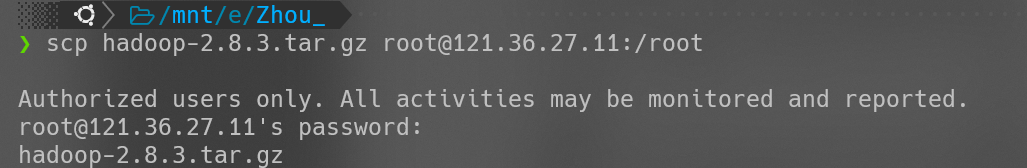
\includegraphics[width = \textwidth]{figure/上传hadoop安装包.png}
                    \caption{上传hadoop安装包}
                    \label{上传hadoop}
                \end{figure}

                将该压缩包解压,并将对应文件移动到正确位置后,使用vim编辑器修改系统配置文件,修改内容如图\ref{修改配置文件}所示。
                \begin{figure}[H]
                    \centering
                    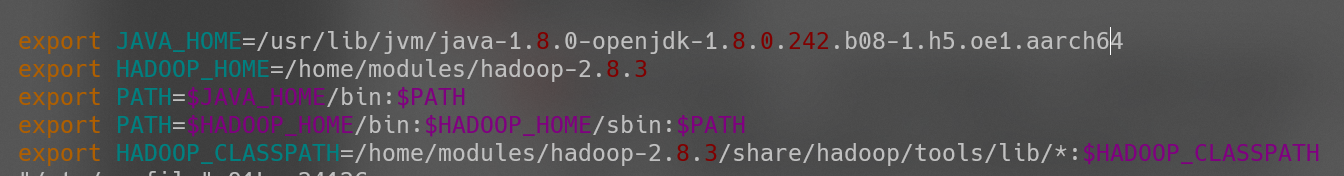
\includegraphics[width = \textwidth]{figure/配置系统环境变量.png}
                    \caption{配置系统环境变量}
                    \label{修改配置文件}
                \end{figure}

                修改好环境变量后进入root目录下验证hadoop安装信息,结果如图\ref{验证hadoop}所示,正确显示了hadoop的版本信息,安装成功。
                \begin{figure}[H]
                    \centering
                    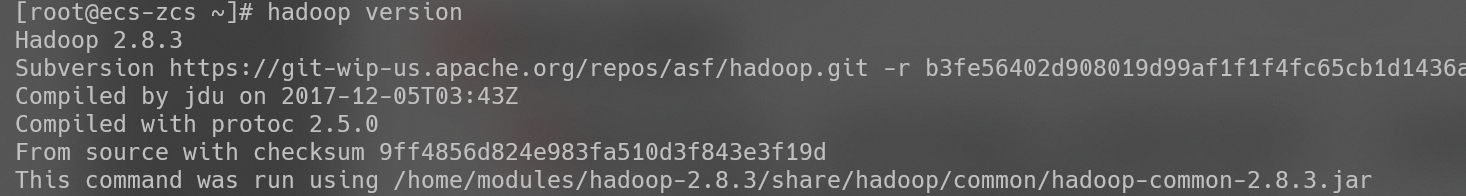
\includegraphics[width = \textwidth]{figure/验证hadoop安装.png}
                    \caption{验证hadoop安装}
                    \label{验证hadoop}
                \end{figure}

            \subsubsection{伪分布式配置}
                配置伪分布式时按照华为官方实验教程进行如图\ref{伪分布式配置}所示步骤
                \begin{figure}[H]
                    \centering
                    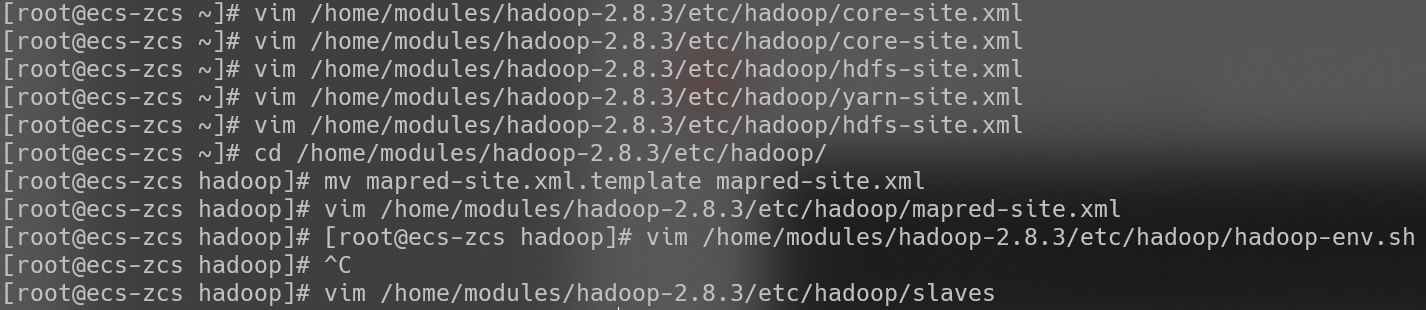
\includegraphics[width = \textwidth]{figure/伪分布式配置.png}
                    \caption{伪分布式配置}
                    \label{伪分布式配置}
                \end{figure}
                在vim中修改了对应的文件之后,即可使用JPS查看运行的进程,查询结果如图\ref{JSP}所示
                \begin{figure}[H]
                    \centering
                    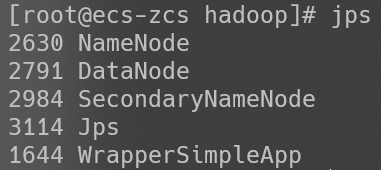
\includegraphics[]{figure/启动HDFS.png}
                    \caption{使用JPS查看启用的进程}
                    \label{JSP}
                \end{figure}

            \subsubsection{Hadoop与OBS互联}
                在上传文件时,我选择了上传自己在另一门课中所编写的Verilog代码的顶层文件,并利用这次的实验原理查询在文件中声明了多少次wire类型的变量(即统计关键词wire的个数)。

                实验过程与华为提供的实验手册操作类似,下载添加jar包的步骤如图\ref{添加jar}所示。
                \begin{figure}[H]
                    \centering
                    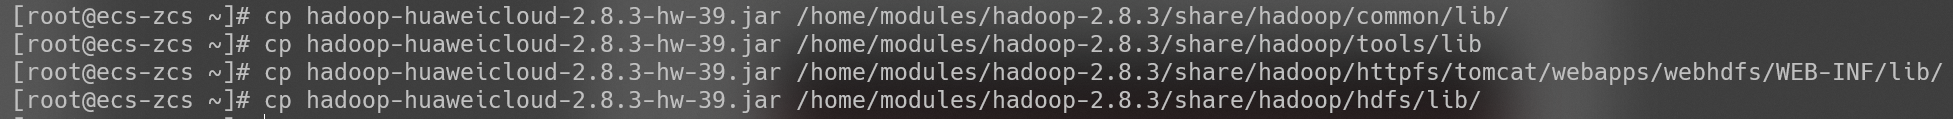
\includegraphics[width = \textwidth]{figure/添加jar包.png}
                    \caption{添加OBSFileSystem相关jar包}
                    \label{添加jar}
                \end{figure}

                随后测试OBS互联,执行HDFS命令查看OBS文件,结果如图\ref{OBS互联}所示:成功查询到了OBS桶中的文件,互联成功。
                \begin{figure}[H]
                    \centering
                    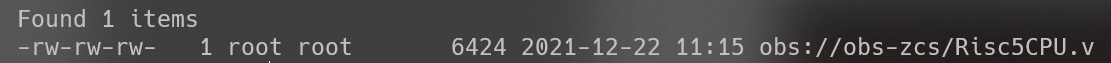
\includegraphics[width = \textwidth]{figure/Hadoop集群与OBS互联成功.png}
                    \caption{测试OBS互联}
                    \label{OBS互联}
                \end{figure}
        
    \section{Spark集群搭建}
        \subsection{实验介绍}
            \subsubsection{关于本实验}
                本部分实验介绍安装Spark集群,并使Spark能够读取OBS数据,使用Python编写Spark程序处理OBS中的数据(单词统计)。该实验使用Spark集群+OBS实现存算分离,提高计算性能。
            \subsubsection{实验目的}
                \begin{enumerate}
                    \item 掌握Spark集群搭建
                    \item 掌握Spark集群与OBS互联
                    \item 使用Python编写Spark程序
                \end{enumerate}
        \subsection{Spark集群存算分离}
            \subsubsection{搭建Spark集群}
                仍旧采用安装hadoop的方法下载好Spark的压缩包,安装实验教程中的方法将其解压、配置相关的jar包,然后配置好Spark的配置文件与系统环境变量,最后是系统环境变量生效。如图\ref{验证Spark的安装}所示,Spark安装成功。
                \begin{figure}[H]
                    \centering
                    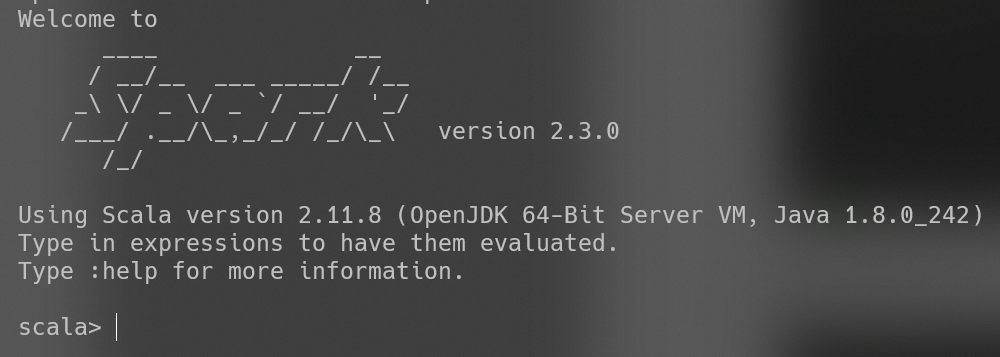
\includegraphics[width = \textwidth]{figure/spark验证完成.png}
                    \caption{Spark安装成功}
                    \label{验证Spark的安装}
                \end{figure}

            \subsubsection{验证存算分离}
            shell编写如Listing \ref{python代码}所示Python代码,即可达到查询出wire个数的目的,查询结果如图\ref{查询结果}所示。
                \begin{lstlisting}[
                    language = python,
                    caption = 验证代码,
                    label = python代码
                ]
# -*- coding:utf-8 -*-
from pyspark.sql.session import SparkSession
spark = SparkSession.builder.getOrCreate()
spark.sparkContext.setLogLevel("WARN")
# 读取OBS数据
lines = spark.read.text("obs://obs-bigdatapro/").rdd.map(lambda r: r[0])
# 统计单词出现次数
counts = lines.flatMap(lambda x: x.split(' ')).map(lambda x: (x, 1)).reduceByKey(lambda x, y: x + y)
output = counts.collect()
# 输出统计结果
    for (word, count) in output:
        if word == 'wire':
            print("%s: %i" % (word, count))
    \end{lstlisting}
    \begin{figure}[H]
        \centering
        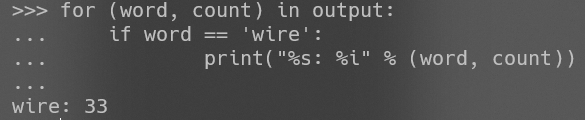
\includegraphics[width = \textwidth]{figure/结果.png}
        \caption{查询结果}
        \label{查询结果}
    \end{figure}

    \section{释放华为云服务}
        如教程所示删除ECS服务器,注意释放弹性公网IP地址。然后删除OBS桶中的对象之后删除OBS桶。

        至此,本次实验结束。

    \section{心得体会}
    这一实验主要是利用华为的弹性云服务器以及OBS桶搭建了一个存算分离的Spark集群。在实验中,数据以对象的形式存储在OBS桶之中,我们通过编写的Python代码使用弹性云服务器访问OBS桶中的数据并弹性云服务器作为算力进行数据分析。
    
    示例中的应用为统计给定文件中各个姓名出现的次数,在了解了整个Spark集群的工作原理之后,我对Python代码进行了小幅度的修改,使其功能变成了统计给定文本中特定单词出现的次数。并利用这一功能统计了自己另一个作业中变量声明的次数。虽然目前看来没有什么大的用处,但是可以预见,当需要分析的数据量变大之后,这一功能的作用也会变得更加的明显。

\end{document}